\chapter{Young Entrepreneur Interviews Shaq}

We should read this lecture as a compact lesson in entrepreneurial mechanics rather than as a loose celebrity interview. Its mathematics is not the mathematics of a blackboard. It is the mathematics of counts, proportions, bargaining room, survival rates, and operational constraints. The lecture begins by giving us answers in compressed form, then resets, then returns to those same answers slowly enough for them to become usable. What finally emerges is a sequence of rules about scale, imitation, retention, hiring, pricing, and durable motive.

\section{The Double Opening: Teaser First, Method Second}

The lecture opens twice. First we are given a fast reel of conclusions: Shaq identifies himself, says he pursued ``a lot'' of industries, is linked to the old fact of owning \(155\) Five Guys locations, gives the one-word answer ``delegation,'' says he did not come from money, names his mother as a motivating force, affirms faith, gives away pizza as an owner who can say yes on the spot, and is then asked about the most money made in a single year. None of this is yet unfolded. It is a preview of doctrine.

Only after that compression does the host reset the scene in Atlanta and tell us what kind of conversation we are entering. Shaq is framed as both one of the greatest basketball players in NBA history and as a business mogul with hundreds of businesses. The host also gives a rough scale marker of wealth, near \(\text{\$}500\) million, though the exact spoken line is slightly garbled in the transcript and should be treated as framing rather than as a theorem of the chapter.

The important thing about this opening is its rhythm. The lecture first spends conclusions and only afterwards supplies the motivating questions. That rhythm should remain visible in the notes. We are not moving from clean definition to clean proposition. We are moving from compressed answers to a slower reconstruction of why those answers matter.

\section{Delegation and the Structure of Scale}

The first clear business principle arrives attached to a number. The host says that Shaq once owned \(155\) Five Guys locations; Shaq says he sold them; then the host asks for the secret of scaling in the franchise model, or in business more generally. Shaq answers with one word: delegation. The explanation is almost embarrassingly simple, and precisely for that reason it is worth formalizing:
\begin{equation}
N_{\text{FG}} = 155.
\end{equation}
The lecture's point is that one person cannot physically inhabit that many locations at once. So the direct form of control fails:
\begin{equation}
1\ \text{owner} \not\Rightarrow N_{\text{FG}}\ \text{locations run directly}.
\end{equation}
What replaces it is distributed execution:
\begin{equation}
\text{delegation} \Rightarrow \text{parallel operators} \Rightarrow \text{scale}.
\end{equation}

This is the chapter's first genuine operator identity. It is not that delegation is merely helpful. It is that beyond a certain count, delegation is the only form in which the enterprise can continue to exist. The arithmetic here is plain, but the commercial consequence is not. A small enterprise can live inside the owner's personal presence. A large one cannot.

\begin{figure}[h]
\centering
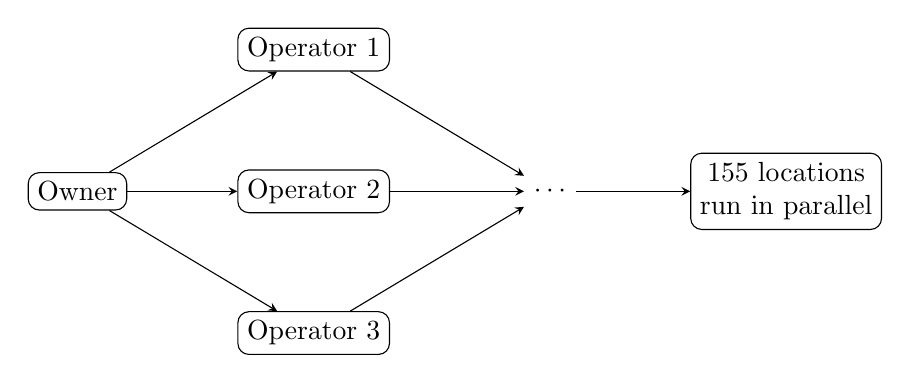
\begin{tikzpicture}[>=stealth]
\node[draw,rounded corners,align=center] (owner) at (0,0) {Owner};
\node[draw,rounded corners,align=center] (d1) at (3,1.8) {Operator 1};
\node[draw,rounded corners,align=center] (d2) at (3,0) {Operator 2};
\node[draw,rounded corners,align=center] (d3) at (3,-1.8) {Operator 3};
\node[align=center] (dots) at (6,0) {\(\cdots\)};
\node[draw,rounded corners,align=center] (loc) at (9,0) {155 locations\\run in parallel};

\draw[->] (owner) -- (d1);
\draw[->] (owner) -- (d2);
\draw[->] (owner) -- (d3);
\draw[->] (d1) -- (dots);
\draw[->] (d2) -- (dots);
\draw[->] (d3) -- (dots);
\draw[->] (dots) -- (loc);
\end{tikzpicture}
\caption{Transcript-based reconstruction of the lecture's scaling claim. The owner does not multiply his body; he multiplies execution through other people.}
\end{figure}

Later in the lecture this same principle returns in a different costume. Shaq says he learned it by winning championships, where great teammates matter. That repetition is not redundancy. It shows that delegation is not an office trick grafted onto business after the fact. It is the same structural habit first learned in competitive team settings and then re-used in enterprise.

\subsection{Question \& Answer}

\paragraph{Question.} How do we scale when one person cannot physically occupy \(155\) places at once?

\paragraph{Answer.} We do not scale by preserving direct presence. We scale by replacing singular presence with distributed competence. In the transcript the replacement word is ``delegation.'' In note form, it is the passage from one body to many operators.

\section{Borrowed Greatness and the Construction of a Self}

After the interview reintroduces Shaq's identity and his many lines of work---DJing, law enforcement, food and beverages, and pizza---the host pivots back to athletics and asks for the biggest driving factor behind his success. Shaq's answer is deliberately provocative: ``I was a thief.'' The lecture then pauses just long enough for him to resolve the provocation: ``Let me explain.''

The explanation is one of the most conceptually sharp moments in the interview. If we see somebody doing better than we are and aspire upward, he says, we should steal what they are doing. The named source set is
\begin{equation}
\mathcal{E}=\{\text{Jordan},\text{Magic},\text{Kareem},\text{Ali}\}.
\end{equation}
He says he took from each of these figures, put those elements inside his brain, and created himself. The resulting map is therefore
\begin{equation}
\mathcal{E} \to \text{internal synthesis} \to \text{constructed self}.
\end{equation}

The chapter should preserve the force of this formulation. The lecture rejects the myth that excellence emerges from pure originality. But it also rejects passive copying. The thief, in Shaq's sense, is not a photocopier. He is a selector and synthesizer. He does not become Michael Jordan or Magic Johnson. He studies them, takes what works, combines those borrowed excellences, and produces a new operator.

This is why the lecture can move, without contradiction, from theft to authorship. What is stolen is method. What is created is a self.

\subsection{Question \& Answer}

\paragraph{Question.} What does Shaq mean by ``steal what they're doing,'' and how does imitation become authorship rather than mere copying?

\paragraph{Answer.} The lecture's answer is that the borrowing is selective. One does not copy a whole person. One extracts working traits from several people, combines them, and builds a usable self out of them. The point is patterned imitation under pressure, not surrender of identity.

\section{Making Money, Keeping Money, and the Missing Vocabulary}

The lecture then pivots from success to the much harsher problem of retention. The host introduces a statistic, attributed in the conversation to Sports Illustrated:
\begin{align}
p_{\text{broke,NFL}} &\approx \frac{1}{3}, &
t_{\text{post-career}} &\approx 3\text{--}5\ \text{years}.
\end{align}
The exact empirical standing of the statistic is less important here than the function it plays in the lecture. It creates the conceptual break between earning and keeping. Shaq answers with the asymmetry directly:
\begin{equation}
\text{easy to make a lot of money} \neq \text{easy to keep a lot of money}.
\end{equation}
That asymmetry is one of the true mathematical statements of the chapter. It says that inflow and preservation are different problems, with different tools and different failure modes.

Pressed on how one preserves large wealth, Shaq names a single technical term: \emph{annuity}. But he refuses to unpack it. He tells the audience to look it up. This refusal is part of the lecture's structure and should not be flattened away. The point here is not that the interview becomes a tutorial on annuity formulas. The point is that financial illiteracy has a vocabulary threshold. There are words one must know before one can even begin to preserve what one has made.

Immediately afterward, the host asks how many businesses he owns. Shaq says he has no idea, and then gives a cautious rhetorical marker while refusing to sound boastful. In that spirit we may record the scale only approximately as
\begin{equation}
N_{\text{biz}} \sim 10^3,
\end{equation}
with the clear caveat that this is rhetoric under self-correction, not a counted ledger. The unresolved question about annual revenue then arrives---and at that precise moment the lecture is interrupted.

\subsection{Question \& Answer}

\paragraph{Question.} Why is keeping money harder than making money once large income arrives quickly?

\paragraph{Answer.} Because the arrival of money does not automatically bring structure, vocabulary, or discipline with it. The lecture's own architecture says this twice: first through the athlete-bankruptcy statistic, and second through Shaq's later autobiographical confession that a first million dollars disappeared almost immediately. Retention is a second education.

\section{The Mid-Lecture Detour and the Arithmetic of Business Practice}

Just when the interview is about to quantify money more precisely, the source breaks away into a long host-side passage on access, mentorship, and entrepreneurial community. This detour is real and should remain visible, but it should remain visibly separate from Shaq's own doctrine. It carries its own scale markers,
\begin{align}
V_{\text{Hilton sale}} &= \text{\$}2.2\ \text{billion}, &
F_{\text{channel}} &> 10\ \text{million},
\end{align}
but these are part of the host's institutional positioning, not part of Shaq's internal chain of business reasoning.

When the interview returns to Shaq, we move into the lecture's most explicit business arithmetic. Asked again about the most money made in a single year, he declines the frame. He says he does not do things for monetary purposes and does not even know how much money he has in today's world. This is not anti-business rhetoric. It is a refusal to let peak income stand in for business method.

The lecture then turns to method. First, it distinguishes starting a business from seeing something already working and doing it. That distinction is paired with a failure-rate heuristic:
\begin{align}
p_{\text{firm failure}} &\approx \frac{8}{10}, &
t_{\text{firm failure}} &\approx 5\ \text{years}.
\end{align}
Again, the point is not statistical finality. The point is that uncertainty is expensive, and proven demand deserves respect.

Second, the lecture adds a social correction: business owners fail when they think they know it all. The operational answer is to hire people smarter than oneself. This sharpens delegation. Delegation is not just about distribution of labor. It is about surrendering the fantasy of personal superiority.

Third, Shaq gives a mentor's retention rule:
\begin{equation}
s = 0.75Y,\qquad c = 0.25Y,\qquad s+c=Y.
\end{equation}
Here \(Y\) is income, \(s\) the saved portion, and \(c\) the portion reserved for enjoyment. The rule is blunt, but blunt rules often survive first contact with money better than elegant ones.

Fourth, and most explicitly, the lecture turns to negotiation. Shaq advises: do not talk first, and start high. The bargaining sequence is presented numerically:
\begin{align}
a_0 &= 200, &
a_1 &= 110, &
a_2 &= 140, &
a_3 &= 125.
\end{align}
Narratively, the sequence is
\begin{equation}
200 \to 110 \to 140 \to 125 \to \text{deal}.
\end{equation}
The lecture then supplies the counterexample that makes the advice vivid. If the other side's budget is
\begin{equation}
B = 200
\end{equation}
and we open at
\begin{equation}
a_0 = 50,
\end{equation}
then the room abandoned at the start is
\begin{equation}
B-a_0 = 200-50 = 150.
\end{equation}

\paragraph{Worked example.}
\begin{enumerate}
\item Let the counterparty's budget be \(B=200\).
\item Let the first ask be \(a_0=50\).
\item The room surrendered immediately is \(B-a_0\).
\item Therefore \(B-a_0=200-50=150\).
\item The lecture's lesson is that a low anchor does not merely sound modest; it destroys negotiating surplus before the bargaining has truly begun.
\end{enumerate}

\subsection{Question \& Answer}

\paragraph{Question.} Why does Shaq tell us not to talk first and to start high?

\paragraph{Answer.} Because the first number functions as an anchor rather than as a polite opening sentence. The lecture's arithmetic shows that if the other side can pay \(200\) and we volunteer \(50\), then the missing \(150\) is not imaginary. It is room surrendered. The point is not theatrical aggression. It is preservation of bargaining space.

\section{Biography Re-entered: Error, Motivation, Faith, and Risk}

The lecture now returns to material that sounds biographical but functions as justification for the rules we have just heard. Delegation comes back first, now tied to championships and great teammates. This return matters. The principle is being shown to have the same shape in sport and business.

Then the background is restated with more weight. Shaq says he did not come from money. He says he saw horror stories about athletes who had nothing a few years after they began playing, and he did not want to become one of those stories. The chapter should let that fear stand, because it provides the emotional pressure behind the later financial rules.

The key mistake is stated vividly:
\begin{equation}
\text{\$}1{,}000{,}000 \to \text{spent in about }30\ \text{minutes}.
\end{equation}
The exact list of purchases in the transcript is slightly garbled, but the quantitative payload is clear. The story is doing real work. It is the lecture's concrete demonstration that scale in earnings can coexist with scale in ignorance, and that structural learning often begins with embarrassment.

The longevity question produces another numerical anchor:
\begin{equation}
t_{\text{NBA}} = 19\ \text{years}.
\end{equation}
The answer is motivational. At first his motive was to get his mother what she wanted. Later, once that had been done, the engine had to be renewed in some other form. The lecture does not formalize the second motive, and it should not be forced into notation. But it does insist on the principle that long performance requires long motive.

Faith enters next, briefly and directly. None of this, he says, is possible without God. The lecture then pivots again, this time to business risk. His biggest risk, he says, was not pulling the trigger when the opportunity was there. Howard Schultz wanted to open Starbucks in neighborhoods Shaq misread. Later, according to Shaq's recollection, Magic Johnson opened roughly
\begin{equation}
N_{\text{Magic Starbucks}} \approx 155
\end{equation}
such stores. The exact count is approximate, but the lesson is precise. Risk is not only losing money by acting. It is also losing opportunity by not seeing the world correctly in time.

From there the lecture becomes a rapid chain of filters. The most successful people are described as nice, humble, simple, and surrounded by strong people. Jeff Bezos becomes the source of an investment rule: invest in things that change people's lives. The pizza episode reappears, again showing ownership through immediate generosity. Then the founder question arrives: what do we look for when investing in a business? Shaq's answer is belief. If the founder's passion is real, he wants to believe in what they believe in.

The next question presses on self-belief, and here the lecture does something subtle. Instead of pretending that willpower alone explains everything, Shaq partially withdraws and attributes much to luck. He had an athletic advantage, was given large amounts of money to play sports, and then leveraged that money into other things. This hesitation improves the lecture. It prevents the notes from turning into motivational sludge. Method survives, but without the pretense that contingency played no role.

The closing blueprint therefore lands with more credibility. If one has a plan, write it down. If someone is already doing what one wants to do, watch them, steal what works, add one's own style, and keep believing through the ups and downs. In compressed form:
\begin{equation}
\text{plan} \to \text{watch what works} \to \text{borrow} \to \text{add style} \to \text{persist}.
\end{equation}

\subsection{Question \& Answer}

\paragraph{Question.} If luck mattered in Shaq's case, what part of the lecture still survives as general method?

\paragraph{Answer.} Quite a lot survives. Delegation, learning from exemplars, hiring above oneself, saving before consuming, respecting proven demand, anchoring high in negotiation, writing the plan down, and persisting through volatility do not disappear when luck is admitted. Luck may affect the scale and timing of the outcome, but it does not abolish the structure of the method.

\section{Summary}

This lecture thinks in a small number of durable shapes. The count \(155\) turns scale into a structural problem. The set \(\mathcal{E}\) turns excellence into selective borrowing. The statistic \(\frac{1}{3}\) over \(3\text{--}5\) years turns money into a retention problem rather than a mere earning problem. The split \(75/25\) turns income into saved and consumed shares. The ladder \(200 \to 110 \to 140 \to 125\) turns negotiation into visible arithmetic. Around these explicit quantities the lecture places its less formal constants: motive, humility, strong people, belief, fear of waste, openness to models, and the refusal to confuse luck with a complete explanation. The result is not a finished theory of wealth. It is something more practical: a grammar of commercial action, learned in public, corrected by error, and kept alive by repetition.